\documentclass[a4paper,12pt]{article}

\input{packages}

\begin{document}

\pagebreak
\section{Les axiomes}
\begin{definition}{Axiome:}
 Un axiome est une proposition admise comme un élément de base d'une théorie mathématique et qui est indémontrable en tant que tel.
\end{definition}

Dans cette section, nous allons définir cinq axiomes, qui nous seront indispensables afin de démontrer des théorèmes par la suite.

\subsection{Axiomes de report (axiomes I et II)}
Le transport des segments et des angles ne change pas leur mesure.

\subsection{Cas d'isométrie des triangles (axiome III)}
Il y a trois cas d'isométrie du triangle. On dit que deux triangles sont isométriques lorsqu'ils sont en tous point semblable, longueurs et angles. Afin de démontrer les deux autres cas d'isométrie des triangles, il faut en prendre un comme axiome.\\

\begin{figure}[H]
    \centering
    \includegraphics[scale=0.6]{axiomes/Cas_1.PNG}
  \end{figure}  
\textbf{Premier cas:} Deux triangles qui ont respectivement un angle et les côtés adjacents isométriques sont isométriques.


\subsection{Axiome de continuité (axiome IV)}
Tout nombre réel positif est la longueur d'un segment. Par exemple, pi peut être représenté comme la moitié du périmètre d'un cercle de rayon 1.
\begin{figure}[H]
    \centerline{\includegraphics[scale=0.4]{axiomes/pi.png}}
    \label{fig:fig2}
\end{figure}

\pagebreak
Ou alors, on peut représenter la racine de deux comme l'hypothénuse d'un triangle rectangle dont les deux côtés valent 1.
\begin{figure}[H]
    \centering
    \includegraphics[scale=0.6]{axiomes/racine2.png}
\end{figure}



\subsection{Axiome des parallèles (axiome V)}
Pour un point donné, il existe une et une seule droite parallèle à une droite et passant par ce point.
\begin{figure}[H]
    \centering
    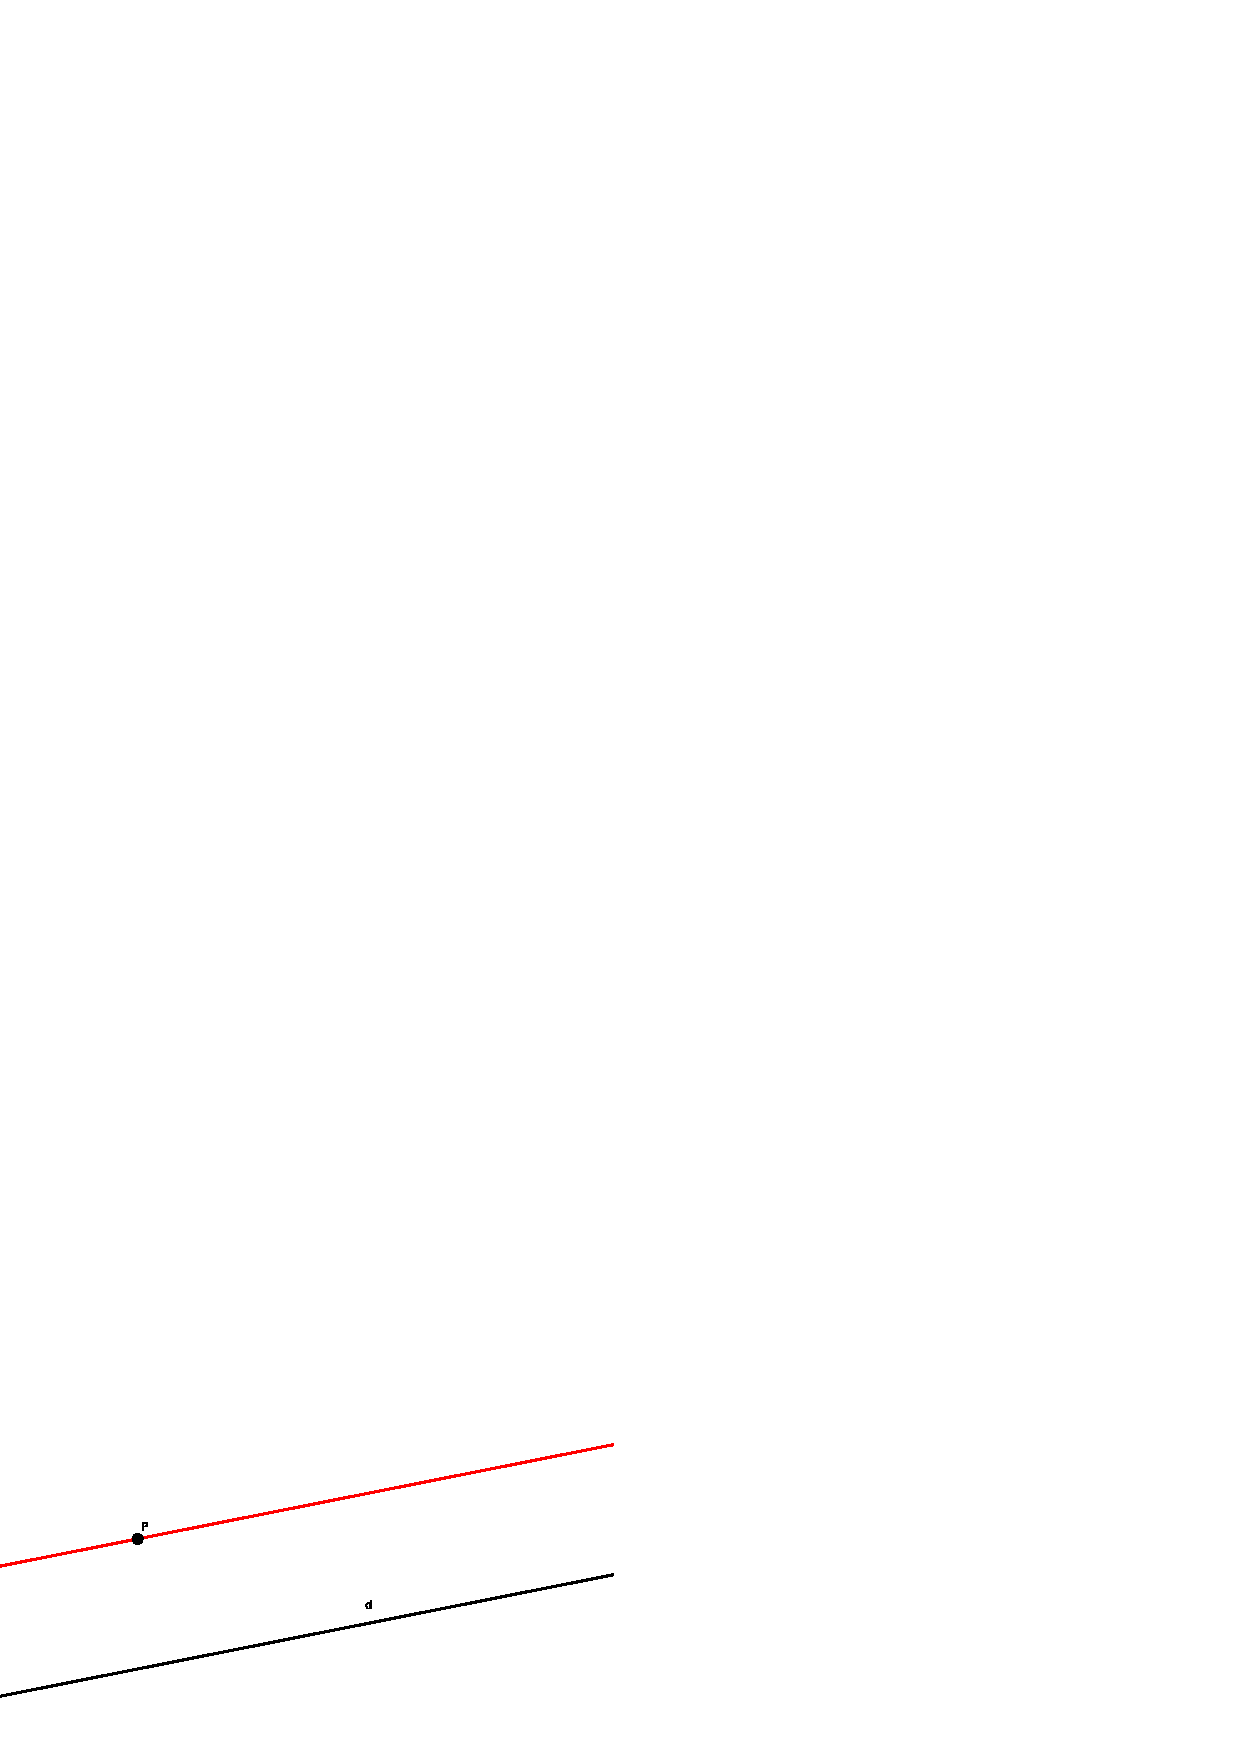
\includegraphics[scale=0.6]{axiomes/parallel.png}
\end{figure}


\end{document}